\documentclass[tikz,border=8pt]{standalone}
\usepackage{amsmath}
\usetikzlibrary{arrows.meta,positioning,fit}

\begin{document}
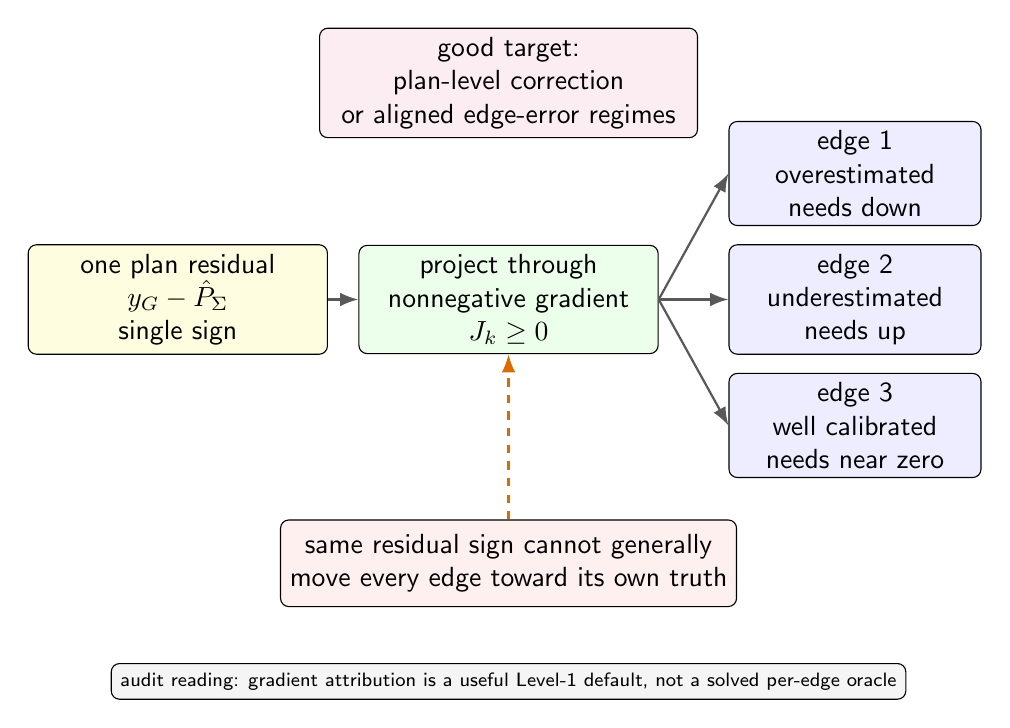
\begin{tikzpicture}[
  font=\sffamily,
  box/.style={draw, rounded corners=3pt, align=center, minimum width=38mm, minimum height=11mm, fill=white},
  edgebox/.style={draw, rounded corners=3pt, align=center, minimum width=32mm, minimum height=9mm, fill=blue!7},
  note/.style={align=center, font=\sffamily\scriptsize},
  arrow/.style={-Latex, thick, draw=black!65},
  warn/.style={-Latex, thick, dashed, draw=orange!85!black}
]

\node[box, fill=yellow!12] (resid) at (0,0)
  {one plan residual\\$y_G-\hat P_\Sigma$\\single sign};
\node[box, fill=green!8] (jac) at (4.2,0)
  {project through\\nonnegative gradient\\$J_k\ge 0$};

\node[edgebox] (e1) at (8.6,1.6) {edge 1\\overestimated\\needs down};
\node[edgebox] (e2) at (8.6,0) {edge 2\\underestimated\\needs up};
\node[edgebox] (e3) at (8.6,-1.6) {edge 3\\well calibrated\\needs near zero};

\draw[arrow] (resid) -- (jac);
\draw[arrow] (jac.east) -- (e1.west);
\draw[arrow] (jac.east) -- (e2.west);
\draw[arrow] (jac.east) -- (e3.west);

\node[box, fill=red!6, minimum width=54mm] (caution) at (4.2,-3.35)
  {same residual sign cannot generally\\move every edge toward its own truth};
\draw[warn] (caution.north) -- (jac.south);

\node[box, fill=purple!7, minimum width=48mm] at (4.2,2.75)
  {good target:\\plan-level correction\\or aligned edge-error regimes};

\node[note, fill=gray!8, draw, rounded corners=3pt, minimum width=90mm] at (4.2,-4.85)
  {audit reading: gradient attribution is a useful Level-1 default, not a solved per-edge oracle};

\end{tikzpicture}
\end{document}
